% Chapter Template

\chapter{Results - Sliding Puzzle} % Main chapter title

\label{Chapter4} % Change X to a consecutive number; for referencing this chapter elsewhere, use \ref{ChapterX}

%----------------------------------------------------------------------------------------
%	SECTION 1
%----------------------------------------------------------------------------------------

\section{Low dimension}

blablabla
%----------------------------------------------------------------------------------------
%	SUBSECTION 1.1
%----------------------------------------------------------------------------------------

\subsection{Perfect Heuristic}

blablabla

%----------------------------------------------------------------------------------------
%	SUBSECTION 1.2
%----------------------------------------------------------------------------------------

\subsection{Results}

blablabla

%-----------------------------------
%	SECTION 2
%-----------------------------------
\section{Intermediary case - 3x3}
\label{S33}
As seen above, we have actually been able to solve the 3 by 3 case perfectly, since it only has 181,440 possible configurations. Its God number is only 31, which definitely makes it manageable. However, this is already an intermediary size, large enough to make trying deep reinforcement learning meaningful.



\begin{landscape}
\begin{figure}[H]
\centering
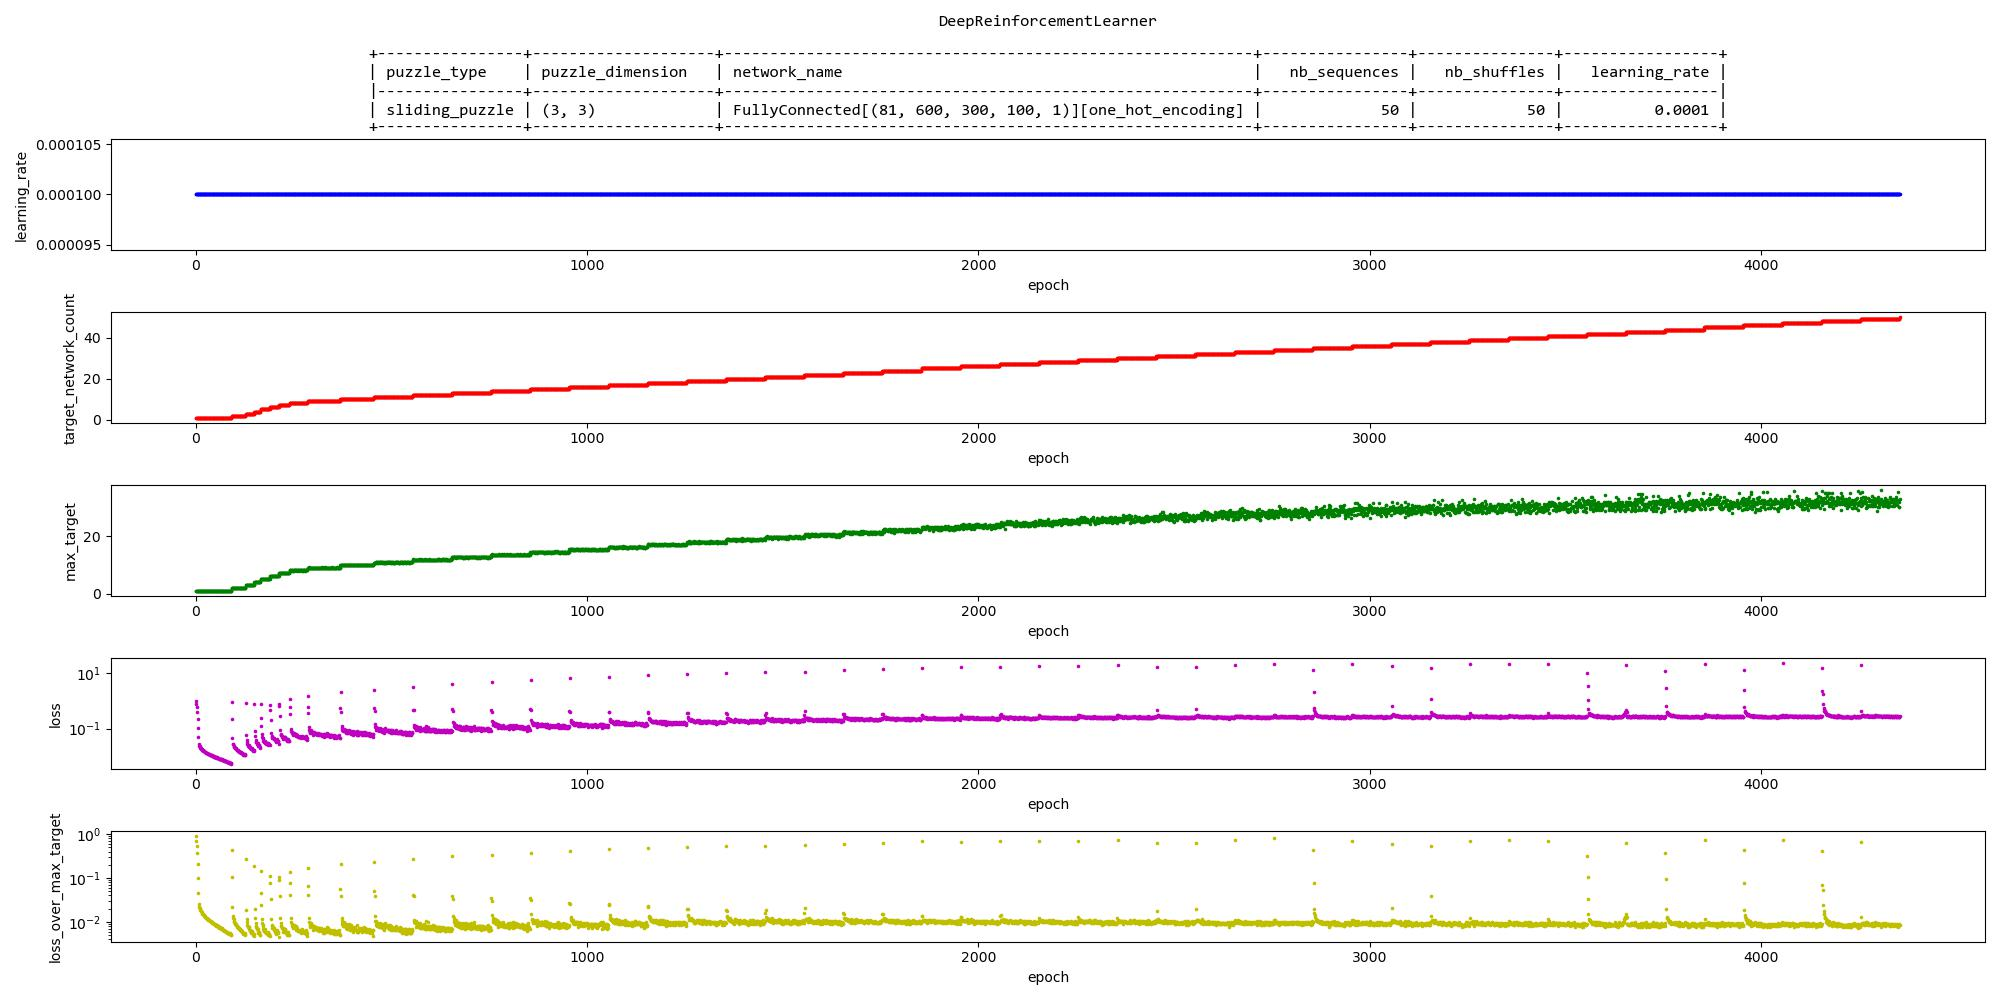
\includegraphics[scale=0.5]{./Figures/33SPDeepReinforcementLearning.jpeg}
%\decoRule
\caption[Codebase]{Code base}
\label{fig:Codebase}
\end{figure}
\end{landscape}


\begin{landscape}
\begin{figure}[H]
\centering
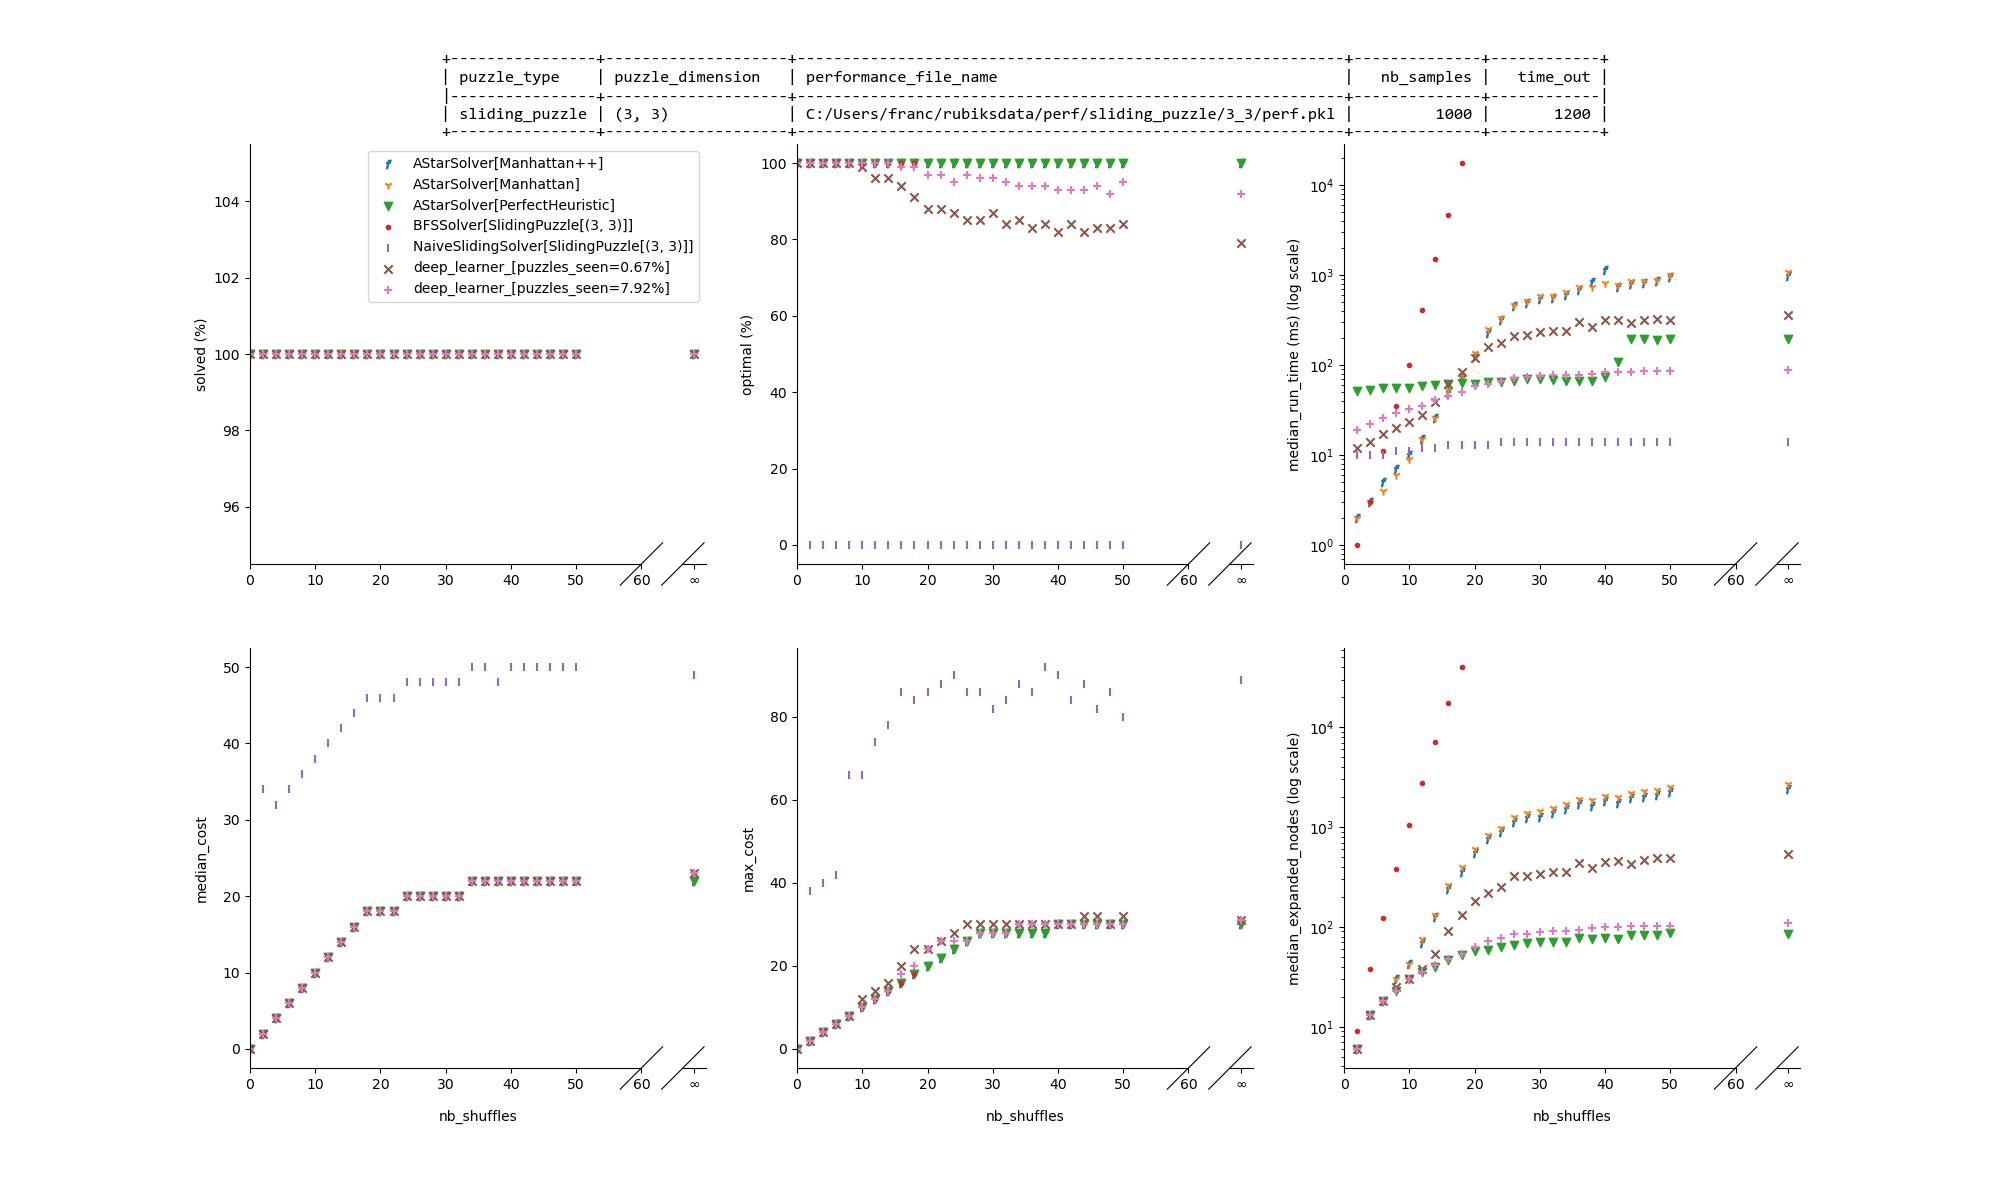
\includegraphics[scale=0.5]{./Figures/33SPPerformance.jpeg}
%\decoRule
\caption[Codebase]{Code base}
\label{fig:Codebase}
\end{figure}
\end{landscape}


%-----------------------------------
%	SECTION 3
%-----------------------------------
\section{3x4}

blabla

%-----------------------------------
%	SECTION 4
%-----------------------------------

\section{4x4}

blabla
